\section{Date: 2026-09-18}
\noindent \textbf{Series ID: BAMLEMHGHGLCRPIUSTRIV} 

\noindent This series is titled ICE BofA High Grade US Emerging Markets Liquid Corporate Plus Index Total Return Index Value and has a frequency of Daily. The units are Index and the seasonal adjustment is Not Seasonally Adjusted.The observation start date is 2023-09-19 and the observation end date is 2026-09-17.The popularity of this series is 2. \\ 

\noindent \textbf{Series ID: CUUR0000SEHF02} 

\noindent This series is titled Consumer Price Index for All Urban Consumers: Utility (Piped) Gas Service in U.S. City Average and has a frequency of Monthly. The units are Index 1982-1984=100 and the seasonal adjustment is Not Seasonally Adjusted.The observation start date is 1935-03-01 and the observation end date is 2026-08-01.The popularity of this series is 9. \\ 

\subsection{Raw Regression}
\noindent Regresses the two series against each other directly. A significant result here can come just as easily from both series sharing a long-run trend as from any real relationship.

\begin{center}
\begin{tabular}{lclc}
\toprule
\textbf{Dep. Variable:}                     & value\_fred\_CUUR0000SEHF02 & \textbf{  R-squared:         } &     0.732   \\
\textbf{Model:}                             &             OLS             & \textbf{  Adj. R-squared:    } &     0.717   \\
\textbf{Method:}                            &        Least Squares        & \textbf{  F-statistic:       } &     49.05   \\
\textbf{Date:}                              &       Fri, 18 Sep 2026      & \textbf{  Prob (F-statistic):} &  1.54e-06   \\
\textbf{Time:}                              &           15:17:42          & \textbf{  Log-Likelihood:    } &   -71.934   \\
\textbf{No. Observations:}                  &                20           & \textbf{  AIC:               } &     147.9   \\
\textbf{Df Residuals:}                      &                18           & \textbf{  BIC:               } &     149.9   \\
\textbf{Df Model:}                          &                 1           & \textbf{                     } &             \\
\textbf{Covariance Type:}                   &          nonrobust          & \textbf{                     } &             \\
\bottomrule
\end{tabular}
\begin{tabular}{lcccccc}
                                            & \textbf{coef} & \textbf{std err} & \textbf{t} & \textbf{P$> |$t$|$} & \textbf{[0.025} & \textbf{0.975]}  \\
\midrule
\textbf{const}                              &     -12.4578  &       36.807     &    -0.338  &         0.739        &      -89.787    &       64.871     \\
\textbf{value\_fred\_BAMLEMHGHGLCRPIUSTRIV} &       1.0247  &        0.146     &     7.004  &         0.000        &        0.717    &        1.332     \\
\bottomrule
\end{tabular}
\begin{tabular}{lclc}
\textbf{Omnibus:}       &  1.439 & \textbf{  Durbin-Watson:     } &    0.633  \\
\textbf{Prob(Omnibus):} &  0.487 & \textbf{  Jarque-Bera (JB):  } &    0.769  \\
\textbf{Skew:}          & -0.480 & \textbf{  Prob(JB):          } &    0.681  \\
\textbf{Kurtosis:}      &  2.969 & \textbf{  Cond. No.          } & 4.45e+03  \\
\bottomrule
\end{tabular}
%\caption{OLS Regression Results}
\end{center}

Notes: \newline
 [1] Standard Errors assume that the covariance matrix of the errors is correctly specified. \newline
 [2] The condition number is large, 4.45e+03. This might indicate that there are \newline
 strong multicollinearity or other numerical problems.

\begin{figure}
\centering
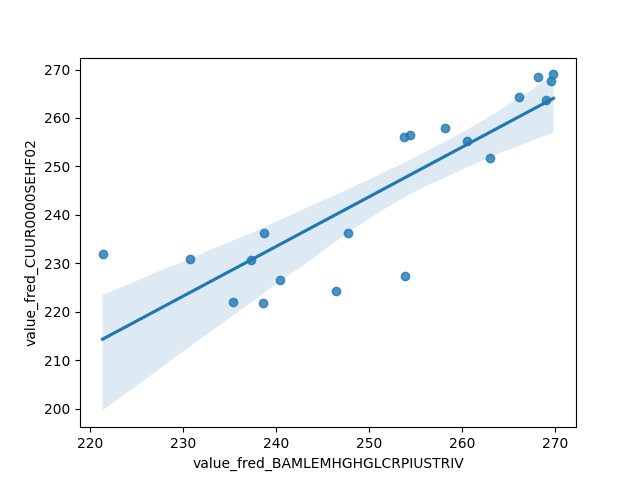
\includegraphics[scale = 0.9]{plots/plot_2026-09-18.png}
\caption{Raw Regression Plot for 2026-09-18}
\end{figure}
\newpage
\subsection{Detrended Regression}
\noindent Regresses the residuals of each series after removing its own linear time trend, so a shared trend can no longer drive the result on its own. A relationship that stays significant here is better evidence of a genuine link between the two series.

\begin{center}
\begin{tabular}{lclc}
\toprule
\textbf{Dep. Variable:}                                & value\_fred\_CUUR0000SEHF02\_detrended & \textbf{  R-squared:         } &     0.056   \\
\textbf{Model:}                                        &                  OLS                   & \textbf{  Adj. R-squared:    } &     0.003   \\
\textbf{Method:}                                       &             Least Squares              & \textbf{  F-statistic:       } &     1.063   \\
\textbf{Date:}                                         &            Fri, 18 Sep 2026            & \textbf{  Prob (F-statistic):} &    0.316    \\
\textbf{Time:}                                         &                15:17:42                & \textbf{  Log-Likelihood:    } &   -66.774   \\
\textbf{No. Observations:}                             &                     20                 & \textbf{  AIC:               } &     137.5   \\
\textbf{Df Residuals:}                                 &                     18                 & \textbf{  BIC:               } &     139.5   \\
\textbf{Df Model:}                                     &                      1                 & \textbf{                     } &             \\
\textbf{Covariance Type:}                              &               nonrobust                & \textbf{                     } &             \\
\bottomrule
\end{tabular}
\begin{tabular}{lcccccc}
                                                       & \textbf{coef} & \textbf{std err} & \textbf{t} & \textbf{P$> |$t$|$} & \textbf{[0.025} & \textbf{0.975]}  \\
\midrule
\textbf{const}                                         &    1.553e-11  &        1.607     &  9.66e-12  &         1.000        &       -3.377    &        3.377     \\
\textbf{value\_fred\_BAMLEMHGHGLCRPIUSTRIV\_detrended} &      -0.4521  &        0.438     &    -1.031  &         0.316        &       -1.373    &        0.469     \\
\bottomrule
\end{tabular}
\begin{tabular}{lclc}
\textbf{Omnibus:}       &  3.477 & \textbf{  Durbin-Watson:     } &    0.858  \\
\textbf{Prob(Omnibus):} &  0.176 & \textbf{  Jarque-Bera (JB):  } &    1.332  \\
\textbf{Skew:}          &  0.090 & \textbf{  Prob(JB):          } &    0.514  \\
\textbf{Kurtosis:}      &  1.749 & \textbf{  Cond. No.          } &     3.67  \\
\bottomrule
\end{tabular}
%\caption{OLS Regression Results}
\end{center}

Notes: \newline
 [1] Standard Errors assume that the covariance matrix of the errors is correctly specified.

\begin{figure}
\centering
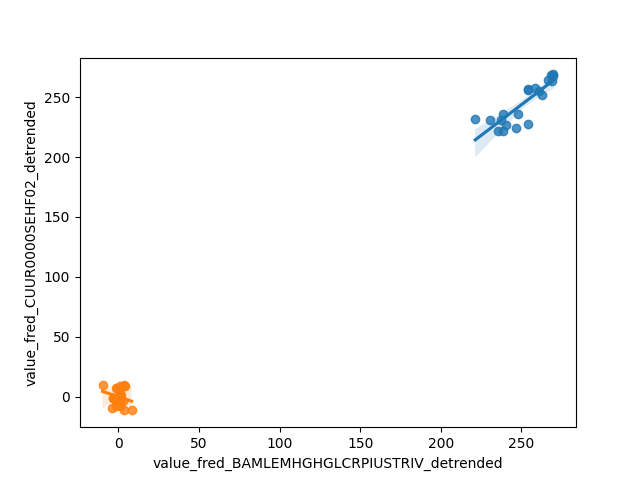
\includegraphics[scale = 0.9]{plots/plot_2026-09-18_detrended.png}
\caption{Detrended Regression Plot for 2026-09-18}
\end{figure}
\newpage
